\section{Admission control}
\label{sec:control}

If the working set will not fit, the server can still choose which sessions hold the memory. Equation~\eqref{eq:gate}
gives the size of the admitted set. We tested four versions of the gate and one published alternative, in the order we
built them; each failure led to the next version. We call them the static gate, the formula, the shared-prefix
formula and the adaptive gate.

\paragraph{A static gate saves energy and starves sessions.} Admitting 16 of 48 synthetic sessions, each for 4 or 8
turns, cut energy per turn by 41--47\% with 5\,s pauses. With 30\,s pauses, where a held slot sits idle for longer, it cost 6--8\% more at 48 sessions and 11--16\%
more at 96. Within a 150\,s step, 6--32 of 48 and 53--80 of 96 sessions were never served. Over 10 minutes, which lets the gate
rotate, the energy gain held, but the latency tail doubled: against the GPU cache alone (333 turns,
1,185\,J per turn, median resume latency 54\,s, 90th percentile 70\,s), the gate gave 456 turns at 761\,J with a median of 1.4\,s
and a 90th percentile of about 146\,s.

\paragraph{The formula and an AIMD window.} Setting $K$ from the engine's reported capacity and the recent size
of sessions, recomputed every 2\,s, saved 40\% and 31\% at 48 and 96 sessions with 5\,s pauses, and 7\% and 1\% with 30\,s pauses. In 150\,s steps it
served only 20 of 48 and 21 of 96 sessions, so part of the gain may have come from serving fewer of them; over 10 minutes at 48
sessions it gave 500 turns at 682\,J, with a median resume latency of 0.5\,s and a 90th percentile of about 147\,s. A CONCUR-style AIMD
window~\cite{chen2026concur}, in our reimplementation with CONCUR's published parameters, saved at most 1.3\% in this
closed-loop setting on synthetic sessions (on recorded trajectories it saved 5\% at 96 sessions and cost 6\% more at
48). On synthetic sessions its window rose to 44 in the first minute, then fell by repeated halving to 1 and stayed
near 1 for the rest of most steps; on recorded trajectories it only grew, to 158, never halving, as did the CONCUR-inspired controller that He
reports~\cite{he2026robot}. This does not test CONCUR itself, whose evaluation is offline batch inference.

\paragraph{Real agents broke the first formula.} Sized from the 90th percentile of recent prompts, the formula admitted
too few recorded SWE-agent sessions: they share a system prompt, which the engine stores once, so the per-session cost
is far below the prompt length. At 192 and 288 sessions it raised energy per turn by 31\% against the GPU cache alone
and served 40--50\% fewer turns. The shared-prefix formula, which subtracts the shared prefix and sizes from the mean (Eq.~\eqref{eq:gate}), reversed
this: $-13\%$ and $-15\%$ against the GPU cache (80.2 and 73.0 against 92.4 and 85.6\,J per turn), with hits 8.5--9.6
points higher and 1.5\% and 8\% fewer turns, repeated within 1.5\% in a second round. On the MoE model, whose GPU cache
never collapsed on these trajectories, the shared-prefix formula changed energy by $+0.3\%$ to $-2.5\%$ and cut the 90th
percentile of resume latency at 192 sessions from 0.37 to 0.22\,s.

\paragraph{A gate next to a host tier.} Combined with a 160\,GB host tier, which on
real trajectories already held 89--91\% of tokens, the shared-prefix formula cost 10\% more energy at 192 sessions and nothing at 288,
against the tier alone, and served 15--18\% fewer turns. We had predicted a further 25\% saving. This run is flawed: its
gate was sized to the GPU's 251k-token capacity instead of the tier's 610k (the trajectory driver preferred the engine's reported capacity to the configured one; the run records the GPU
value), so it
admitted a median of about 100 sessions at a time (24--280 over a step) of the 192--288 open; it shows only that a gate sized to the GPU should not front a host tier. On synthetic sessions, where the tier alone reached only
35\% hits at 96 sessions over 10 minutes, the original (90th-percentile) formula with a 160\,GB tier, sized to the tier, cut energy per turn by 36\% with 34.5\% more turns,
served all 96 sessions and moved the median resume latency from 110\,s to 16\,s at the price of a longer tail (204\,s
against 124\,s at the 90th percentile). A gate helps only when memory is short.

\paragraph{An adaptive gate.} The last version applies $K$ only when the open sessions' working set exceeds
$\theta C$ with $\theta=1.2$, and otherwise admits everyone. We registered its predictions before running it on two
workloads, two rounds each (Table~\ref{tab:adaptive}, Figure~\ref{fig:adaptive}). Below the cliff it matched the GPU cache in energy (within
0.2\% at 4 and 8 long-context sessions) and in latency (on Qwen3-8B at 64 sessions the switch turned the gate on in
about a fifth of its 2\,s control intervals, so a few resumed turns waited up to 17\,s for readmission); the formula alone had cost up to 2.7\% more energy at long context and, on
Qwen3-8B at 64 sessions, used 9\% less energy than the GPU cache but had a 90th-percentile resume latency of 8--12\,s instead of 1.6--1.9\,s. Above the cliff it took the full
gain of the formula: 41\% less energy per turn on Qwen3-8B at 128 and 256 sessions and 44--45\% at 16 and 32
long-context sessions, with 90th-percentile resume latency falling from 24--81\,s to 0.6--1.5\,s and from 40--121\,s to
8.7--12.7\,s. Every registered threshold held. At 4 and 8 long-context sessions the switch never turned the gate on, so
those cells ran as the GPU cache; the switch changed state only on Qwen3-8B at 64 sessions. We did not test $\theta=1.2$ with
30\,s pauses, where hits persist to $W/C\approx1.86$, nor on recorded or production traffic.

\begin{figure*}[t]
\centering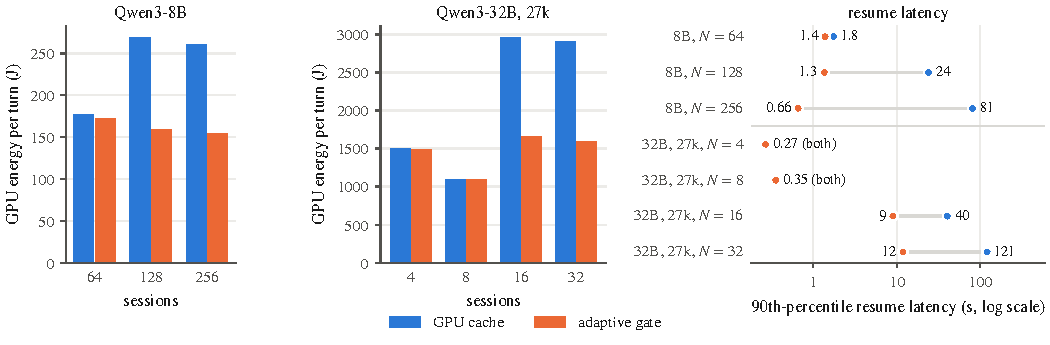
\includegraphics[width=\textwidth]{../figures/adaptive.pdf}
\caption{The adaptive gate against the GPU cache alone, for both workloads of Table~\ref{tab:adaptive} (vLLM, 5\,s
pauses, 150\,s steps). Left and middle: measured GPU energy per turn, mean of two rounds (the two rounds agree within 1.5\% in
every cell). Right: 90th percentile of resume latency, one row per cell (mean of two rounds; turns after a session's
first), including any wait for admission, on a log scale. Below the cliff (8B at 64 sessions, 32B at 4 and 8) the two policies are within 3\% in energy; above
it the gate cuts energy by 41--45\% and the tail of resume latency by 4.5--123$\times$;
first admissions wait longer and fewer sessions are served at the highest loads (Section~\ref{sec:control}).}
\label{fig:adaptive}
\end{figure*}

These latency figures, like the registered thresholds, cover resumed turns; admission waits fall mostly on first
turns. Above the cliff the 90th percentile of first-turn latency was 88--91\,s and 130\,s with the gate on Qwen3-8B at
128 and 256 sessions (38 and 88\,s with the GPU cache alone) and 112--113 and 110--114\,s at 16 and 32 long-context sessions (62
and 132\,s): longer in three of the four cells over the sessions served, and in all four once the sessions never served,
each waiting at least 143\,s, are counted. At the two highest loads the gate served only 170 of 256 and 16--17 of 32 sessions within the 150\,s step,
where the GPU cache served all of them, so part of its energy gain there may come from serving fewer sessions, as with
the static gate (in 600\,s steps, with every session served, the gain held). Over all turns of the sessions served, its 90th-percentile latency was 68--86\,s against 30--82\,s
for the GPU cache on Qwen3-8B and 77--82\,s against 54--122\,s at long context. 
\paragraph{Ten-minute steps.} To see whether rotation closes this gap, we registered a further prediction (H28)
and ran the gate and the GPU cache for 600\,s at the two loads where sessions went unserved, one round, on a second
H200 NVL host with the same engine and meter versions (Table~\ref{tab:tenmin}); a third registered cell, Qwen3-8B at 128 sessions, was
dropped for budget reasons before any data were collected. The 10-minute baselines, on the second host, used more energy per turn than the 150\,s baselines on the first (292 against
261\,J on Qwen3-8B, 3,022 against 2,901\,J at long context). With rotation the gate served every session,
completed 48\% and 62\% more turns and cut energy per turn by 42\% and 50\%; no session completed fewer turns than
under the GPU cache. The cost is queueing: the 90th percentile of first-turn latency was 183 against 68\,s and 253
against 131\,s, and of resumed turns including readmission waits 226 against 102\,s and 251 against 130\,s. H28's
energy and served-sessions clauses held; its latency clause (at most 1.5 times the GPU cache's first-turn tail) did
not. In these two 10-minute runs the gate traded first-turn latency, rather than sessions served, for throughput and energy.


\begin{table}[t]
\centering\small
\caption{The adaptive gate against the GPU cache alone (vLLM, 5\,s pauses, 150\,s steps, two rounds). $N$: sessions. J/turn: energy per turn, mean of the two rounds. p90: 90th
percentile of resume latency (turns after a session's first) including any wait for admission, as a range over the two rounds, or one value where they agree at the precision shown.}
\label{tab:adaptive}
\setlength{\tabcolsep}{3pt}
\begin{tabular}{lrrrrr}
\toprule
Workload & $N$ & \multicolumn{2}{c}{J/turn} & \multicolumn{2}{c}{p90} \\
\cmidrule(lr){3-4}\cmidrule(lr){5-6}
 & & GPU & adaptive & GPU & adaptive \\
\midrule
Qwen3-8B & 64 & 176.6 & 171.9 & 1.6--1.9\,s & 1.3--1.5\,s \\
Qwen3-8B & 128 & 269.6 & 159.6 & 24\,s & 1.2--1.5\,s \\
Qwen3-8B & 256 & 261.3 & 154.5 & 81\,s & 0.6--0.7\,s \\
Qwen3-32B, 27k & 4 & 1,495 & 1,494 & 0.27--0.28\,s & 0.26--0.28\,s \\
Qwen3-32B, 27k & 8 & 1,095 & 1,094 & 0.35--0.36\,s & 0.35--0.36\,s \\
Qwen3-32B, 27k & 16 & 2,964 & 1,658 & 40\,s & 8.7--9.2\,s \\
Qwen3-32B, 27k & 32 & 2,901 & 1,589 & 121\,s & 11.0--12.7\,s \\
\bottomrule
\end{tabular}
\end{table}

\begin{table}[t]
\centering\small
\caption{The adaptive gate in 600\,s steps (vLLM, 5\,s pauses, one round, second host). $N$: sessions. Served: sessions with at
least one turn. Min.\ turns: fewest turns any session completed. p90 first: 90th percentile of first-turn latency including
admission waits. Gate: the adaptive gate.}
\label{tab:tenmin}
\setlength{\tabcolsep}{2.4pt}
\begin{tabular}{lrlrrrrr}
\toprule
Workload & $N$ & Policy & Served & Turns & J/turn & Min. & p90 \\
 & & & & & & turns & first \\
\midrule
Qwen3-8B & 256 & GPU & 256 & 1,436 & 292 & 5 & 68\,s \\
 & & gate & 256 & 2,119 & 168 & 6 & 183\,s \\
Qwen3-32B, 27k & 32 & GPU & 32 & 143 & 3,022 & 4 & 131\,s \\
 & & gate & 32 & 232 & 1,507 & 4 & 253\,s \\
\bottomrule
\end{tabular}
\end{table}

The adaptive gate is a working-set admission rule with a switch; it is not a new idea in kind (Section~\ref{sec:related}).
The measurements show where each part helps: the shared-prefix term on real agents, the switch below the cliff, where it keeps latency at the GPU cache's level, and
the formula above it, with its gain in joules and its cost at admission. A correctly sized gate next to a host tier
that already holds the working set remains untested on real trajectories.
